% Rešerše – ABRA (vkládá se do kapitoly 01-reserse.tex)
\section{ABRA}\label{sec:reserse-abra}

Společnost ABRA Software nabízí dva produkty: ekonomický systém \emph{ABRA Flexi} (dříve FlexiBee) pro malé a~střední firmy a~ERP \emph{ABRA Aiva} pro střední a~velké firmy. Pro srovnání byla zvolena ABRA Flexi, která jako jediná nabízí zkušební verzi a~cílí na menší firmy. Základní údaje shrnuje tabulka~\ref{tab:reserse-abra}.

\begin{table}[H]
\centering
\small
\begin{tabular}{>{\raggedright\arraybackslash}p{0.24\linewidth}>{\raggedright\arraybackslash}p{0.70\linewidth}}
\hline
\textbf{Kritérium} & \textbf{Zjištění} \\
\hline
Název & ABRA Flexi (pro větší firmy ABRA Aiva) \\
Společnost & ABRA Software s.r.o., Praha (CZ); přibližně 35 let na trhu, přes 7~300 zákaznických firem \cite{abra-web} \\
Typ aplikace & webová aplikace a~desktopový klient pro Windows, Linux i~macOS \cite{abra-flexi-cenik} \\
Hostování & primárně cloud výrobce (Amazon Web Services); vlastní server je možný jen s~placenou rozšířenou podporou \cite{abra-flexi-cenik} \\
Licence & proprietární, předplatné bez vstupního poplatku \cite{abra-web} \\
Cena & za pojmenovaného uživatele a~měsíc při měsíční / roční platbě: Basic 425 / 390~Kč, Business 1~055 / 967~Kč, Premium 1~375 / 1~260~Kč; uživatelé pouze pro čtení zdarma; ABRA Aiva jen na poptávku, nasazení v~řádu stovek tisíc až milionů korun \cite{abra-flexi-cenik,abra-aiva-cena} \\
Zkušební verze & 30 dní všech tarifů, bez platební karty \cite{abra-flexi-cenik} \\
\hline
\end{tabular}
\caption{Základní údaje o~řešení ABRA}\label{tab:reserse-abra}
\end{table}

\subsection{Zkušenosti ze zkušební verze}

První dojem z~aplikace je velmi pozitivní, systém působí všestranně. Hned při založení účtu lze nastavit vzhled aplikace a~velikost písma, takže rozhraní je přehledné a~čitelné. Pro vyzkoušení si lze nechat vygenerovat ukázková data. Úvodní nástěnka zobrazuje souhrny a~grafy, které jsou příjemné, ale pro potřeby servisní firmy nejsou podstatné. Navigace je stejně jako u~iDokladu v~levém panelu, který lze zúžit jen na ikony. Modré tlačítko \emph{Nový} v~pravém horním rohu je dobře viditelné a~odlišené od ostatních prvků, formuláře mají v~pravém dolním rohu jednotná tlačítka \emph{Zavřít} a~\emph{Uložit a~zavřít}. Sekce \emph{Všechny agendy} umožňuje připnout si do menu jen potřebné části systému, což odpovídá myšlence navrhované aplikace, tedy funkčnímu jádru s~volitelnými rozšířeními.

Tabulky (adresář firem, vydané faktury) jsou jednotné a~přehledné, ale ve výchozím stavu zobrazují velké množství sloupců. Lze si nastavit zobrazené sloupce i~uložit vlastní pohledy, což je dobrý nápad, avšak pro malou firmu zbytečně složitý; po každé změně filtru či řazení navíc aplikace nabízí uložení pohledu. Filtrování se otevírá v~postranním panelu, který zbytek obrazovky zašedne. Detail záznamu se otevře jen kliknutím na sloupec \emph{Interní číslo}, nikoli na celý řádek, což není na první pohled patrné. Stav úhrady je zobrazen procentem zaplacené částky místo srozumitelného stavu (odesláno, zaplaceno). Inspirativní je naopak souhrn počtu dokladů a~jejich celkové částky ve spodní části tabulky. Formulář nové firmy obsahuje velké množství polí; pro potřeby servisní firmy by stačila základní část s~kontaktní osobou a~přílohami. Pozitivně lze hodnotit i~systém upozornění, který se zapíná v~nastavení a~nezakrývá obsah obrazovky. Globální vyhledávání v~horní části je naopak příliš obecné a~často vede do nastavení místo k~hledanému záznamu.

Zásadní rozdíl je v~pojetí zakázky (obrázek~\ref{obr:abra-zakazka}). Zakázka v~ABRA Flexi je chápána jako obchodní příležitost s~předpokládanými náklady a~ziskem, nikoli jako evidence přijatého zařízení a~průběhu opravy. Nabídky, objednávky a~zakázky jsou navíc dostupné až v~tarifu Business za 1~055~Kč za uživatele měsíčně. Tisk dokumentů nabízí výběr tiskové sestavy, možnost upravit vzhled dokumentu podle vlastní šablony se však v~uživatelském rozhraní nepodařilo najít, přestože nápověda popisuje konfigurovatelné reporty pro vybrané doklady \cite{abra-flexi-reporty}. Evidence zařízení, provedené práce a~kalendář v~systému chybí a~materiál je řešen pouze jako sklad.

\begin{figure}[H]
\centering
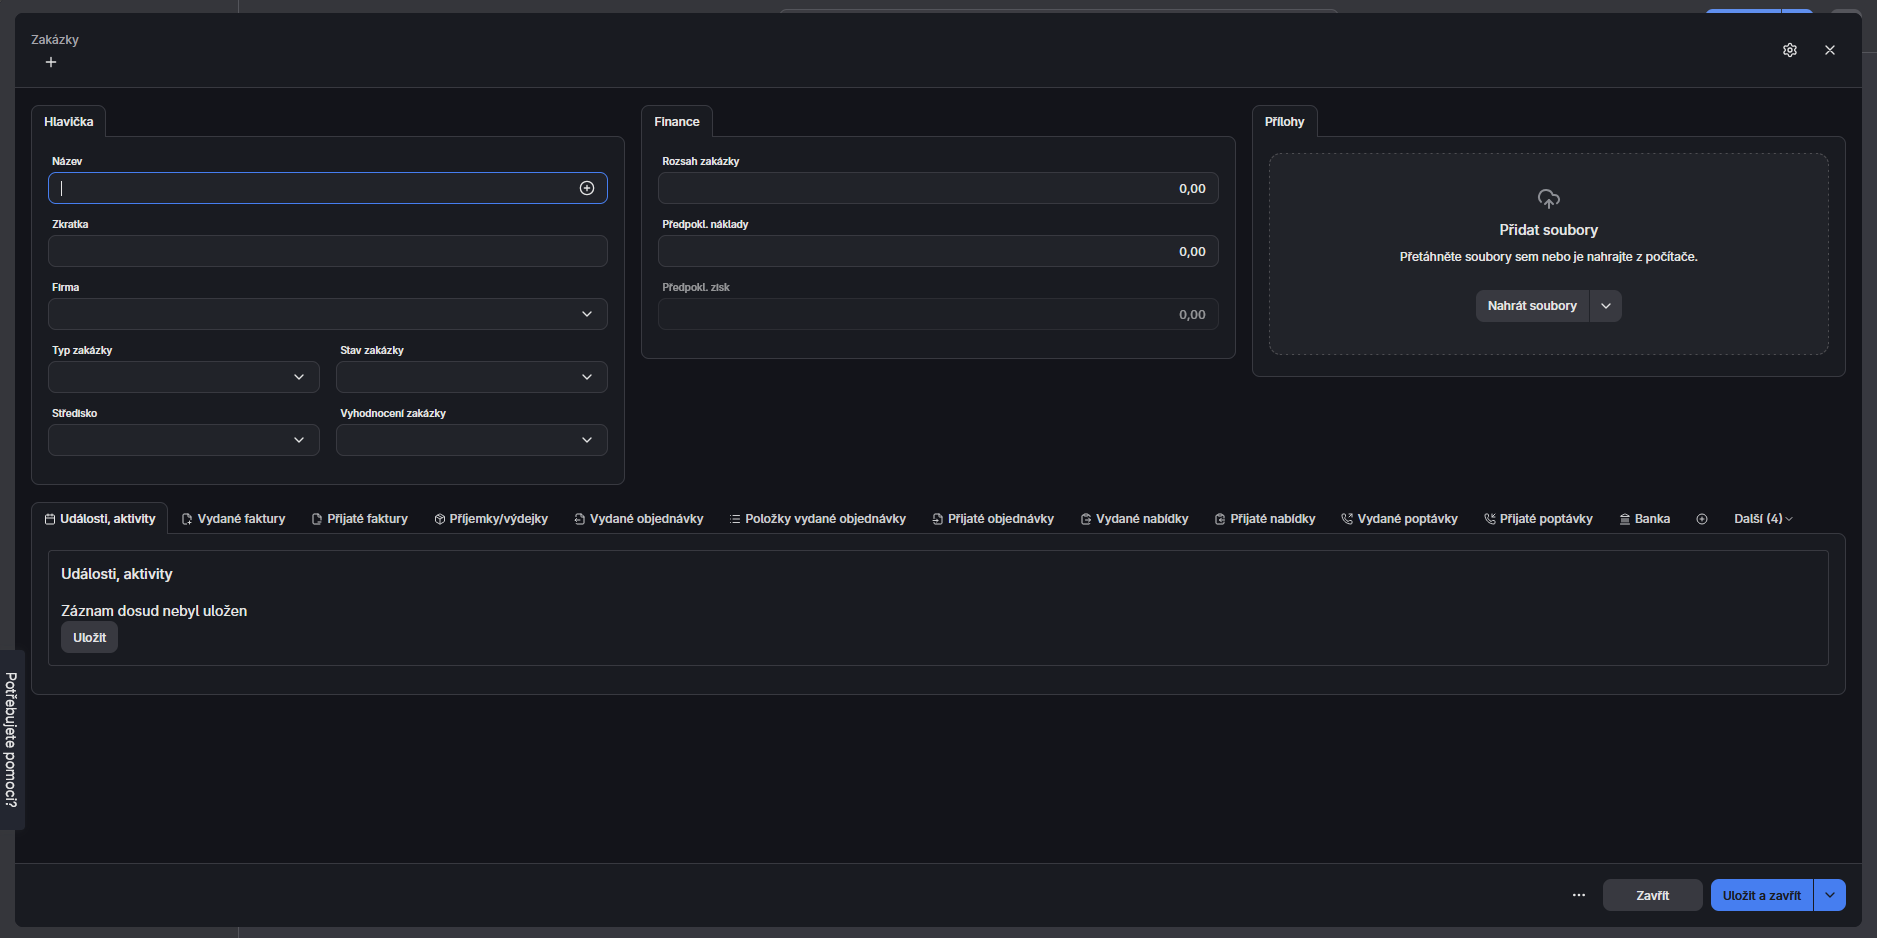
\includegraphics[width=\linewidth]{obrazky/reserse/abra_pridani_zakazky.png}
\caption{Formulář nové zakázky v~ABRA Flexi: zakázka je pojata jako obchodní případ s~rozsahem, náklady a~ziskem (zdroj: vlastní snímek obrazovky ze zkušební verze, pořízeno 3.~11.~2026)}\label{obr:abra-zakazka}
\end{figure}

\subsection{Vhodnost pro malé firmy}

ABRA Flexi je vhodná pro malé firmy, které chtějí vést kompletní účetnictví a~daňovou evidenci samy. Pro malou servisní firmu však nemá přiměřený poměr ceny a~přínosu: tarif Basic obsahuje z~potřebných funkcí v~podstatě jen fakturaci, kterou levněji nabízejí fakturační nástroje, a~tarif Business, který se potřebám firmy blíží nejvíce, stojí přes 1~000~Kč za uživatele měsíčně, a~přesto neobsahuje servisní evidenci. Rozhraní je přehledné a~přizpůsobitelné, ale orientované na zkušené administrativní a~účetní pracovníky.
